%% CHAPTER 2
% Initialization of the system
%  - Analysis of the image in the HSV space
%  - Writing down the classifier. Implementing it in class ParkSpot

\section{Initialization of the System}

	\subsection{Classification with Histograms}
	
	Here is presented the algorithm used to initialize the system. The algorithm is
	a classifier developed upon the classification of two main parameters that
	tends to separate busy parking spot, from free ones. 
	
	Taken an image converted in HSV color space, we could extract the mean and the
	standard deviation for each component. The plot of the standard
	deviation of the Saturation components against the mean of Value component, for
	a single frame, will give us this single situation. Parking spot status is
	known, and we can see a strong separation (see figure \ref{fig:separate}, on
	the left).
	
	The two different status could be separated with two degrees of freedom of a
	line. The inclination and offset of the line could be used to derive
	rotation plus translation equation that will help us to discriminate between
	the busy and the free parking spot. Given a point ${\sigma_{2},\mu_{3}}^{T}$, and a
	separation line in the form $\mu_{3} = \alpha \sigma_{2}+\eta$, we could derive
	this transformation:
	\begin{equation}
		\left\{ \begin{array}{c}
\xi_{1}\\
\xi_{2}
\end{array}\right\} =\left[\begin{array}{cc}
\cos(\alpha) & \sin(\alpha)\\
-\sin(\alpha) & \cos(\alpha)
\end{array}\right]\left\{ \begin{array}{c}
\sigma_{2}\\
\mu_{3}
\end{array}\right\} -\left\{ \begin{array}{c}
1\\
1
\end{array}\right\} \eta
	\end{equation}
	the algorithm has only to check:
	\begin{equation}
		\xi_{2} \geq 0
	\end{equation}
	if this condition is true, than the park spot is busy, else the parking spot is
	free.
	% TODO Figura separazione singola e rispetto al tempo label: fig:separate
	\begin{figure}[H] \label{fig:separate}
		\centering
			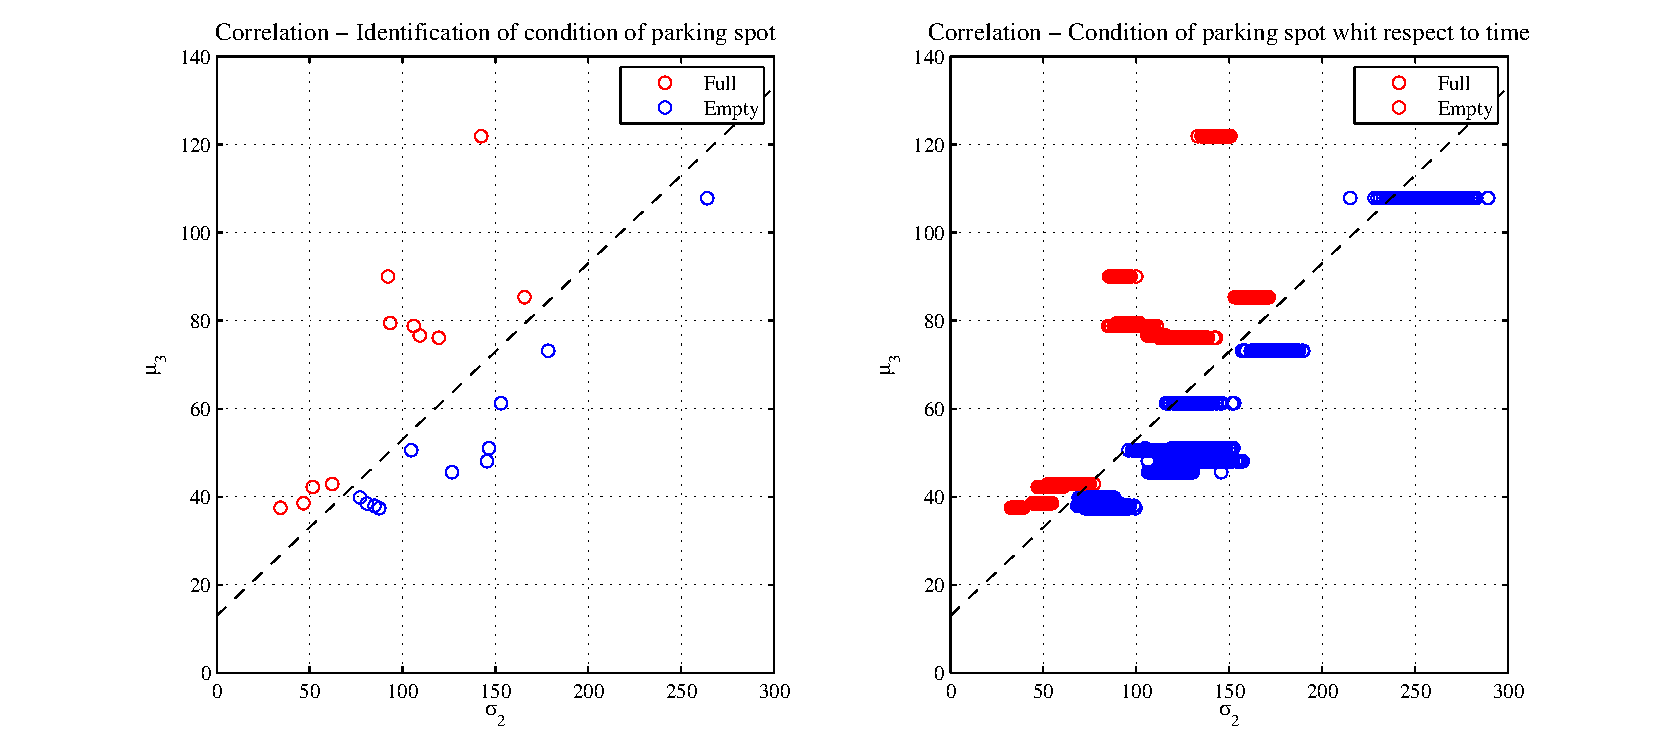
\includegraphics[keepaspectratio, scale=0.4]{img/img1.pdf}
		\caption{Classifier data in 2D representation}
	\end{figure}
	
	Referring to the image on the right, in figure \ref{fig:separate}, it is easy
	to understand that this classification is not robust in time, if not
	expanded with tuning of the parameters each frame (learning
	algorithm). Means tend to remain almost equal, but standard deviations tend to
	change in time. The learning method should change the angle of the separation
	line (and also the discrimination algorithm) to get a good classification. We
	have decided to leave this method, for something that is little more 
	sophisticated, and to discover more about the \verb+openCV+ libraries.
	
	As a drawback, we can also consider the fact that there will be no control on
	the evolution of the classifier discrimination parameters.
	
	\subsection{Diving in the Code}
	In the code, this initialization script is called when a new object
	\verb+ParkSpotObj+ is created, as \verb+int ParkSpotObj::initialStatus()+
	method. The projection of the two characteristics is made by the single object,
	to follow the self-containment philosophy. The parameters that drive the
	algorithm are the number 3 and 4 in the \verb+param+ element of the
	configuration script.
	
	The code is almost at a good level of optimization, because the number of bins
	extracted for the histograms are 32, and the area on which is evaluated the
	status is relatively small.
